\chapter{System Design and Implementation} \label{ch:problem-solution}

This chapter presents the design and implementation of the Pista system to address the challenges identified in startup pitch evaluation. The fundamental aspects of the system architecture are explained, along with the technical decisions made during development, and how each component works together to provide consistent, GenAI-powered startup evaluations.

The chapter is organized around the key technical elements that make Pista work. The chapter is structured to first explain the solution approach and design philosophy, followed by the system architecture, technical implementation, and finally, the performance characteristics and deployment approach

\section{Solution Approach and Design Philosophy} \label{sec:solution-approach}

The Pista system was designed to solve three main problems in startup pitch evaluation: inconsistency between different evaluators, limited access to expert-level assessment, and scalability challenges. These problems were addressed by creating a system that uses GenAI to provide standardized evaluations based on research-backed criteria.

The core design philosophy focuses on evidence-based assessment rather than subjective opinions. Traditional pitch evaluations often vary widely because different evaluators focus on different aspects or use different standards. Pista addresses this by using a fixed evaluation framework with clear criteria and requiring evidence to support higher scores.

The system was built around four key design principles. First, the evaluation framework uses standardized criteria derived from venture capital research to ensure assessments focus on factors that actually predict startup success. Second, the system requires concrete evidence for all scoring decisions to prevent unsupported claims from receiving high ratings. Third, the architecture prioritizes simplicity and reliability over complex features to maintain research data quality. Fourth, the user interface guides users through a consistent process while presenting results in a clear, structured format.

The system processes a startup pitch, which can be either text or audio. It generates targeted questions to fill information gaps, processes the content through a structured evaluation framework, and then returns both numeric scores and detailed qualitative feedback. This approach combines the speed and consistency of automated assessment with the depth and insight that entrepreneurs need for improvement.

\section{System Architecture and Technical Implementation} \label{sec:system-design}

This section explains how the technical architecture was built to support reliable GenAI-powered evaluations. The overall architecture design, evaluation framework implementation, GenAI integration, data models, and API structure are covered.

\subsection{Architecture Overview}\label{subsec:architecture-overview}

Modern web technologies were selected that work well together for rapid development while supporting the real-time features needed for research applications. The architecture uses Next.js 15 with React for the frontend, Convex for the database and backend functions, and OpenAI's API for GenAI processing.\footnote{The complete technology stack includes: Next.js 15 (React framework), TypeScript (type safety), Tailwind CSS (styling), Shadcn/ui (UI components), Convex (backend-as-a-service), Clerk (authentication), OpenAI API (GPT-4 and Whisper), Zustand (state management), Vitest (testing), and React Testing Library (component testing).} This technology stack was chosen after evaluating alternatives based on development speed, real-time capabilities, and research data reliability. The combination provides server-side rendering for fast page loads, real-time synchronization for evaluation updates, and robust API integrations for GenAI processing. TypeScript was used throughout the implementation to ensure type safety and reduce runtime errors, which is critical for maintaining research data integrity.

Figure~\ref{fig:user-flow} shows the complete user workflow and how data moves through the system. Users can upload either text pitches or audio files, which the system processes through transcription (if needed), question generation, evaluation, and results storage. The workflow was designed to handle both synchronous and asynchronous operations, with audio transcription running separately from evaluation processing to prevent interface blocking. Real-time progress updates are provided throughout each step using Convex's reactive query system, allowing users to monitor processing status without manual page refreshes. This architecture ensures consistent data flow regardless of input type while maintaining responsive user experience during computationally intensive operations.

\begin{figure}[H]
  \centering
  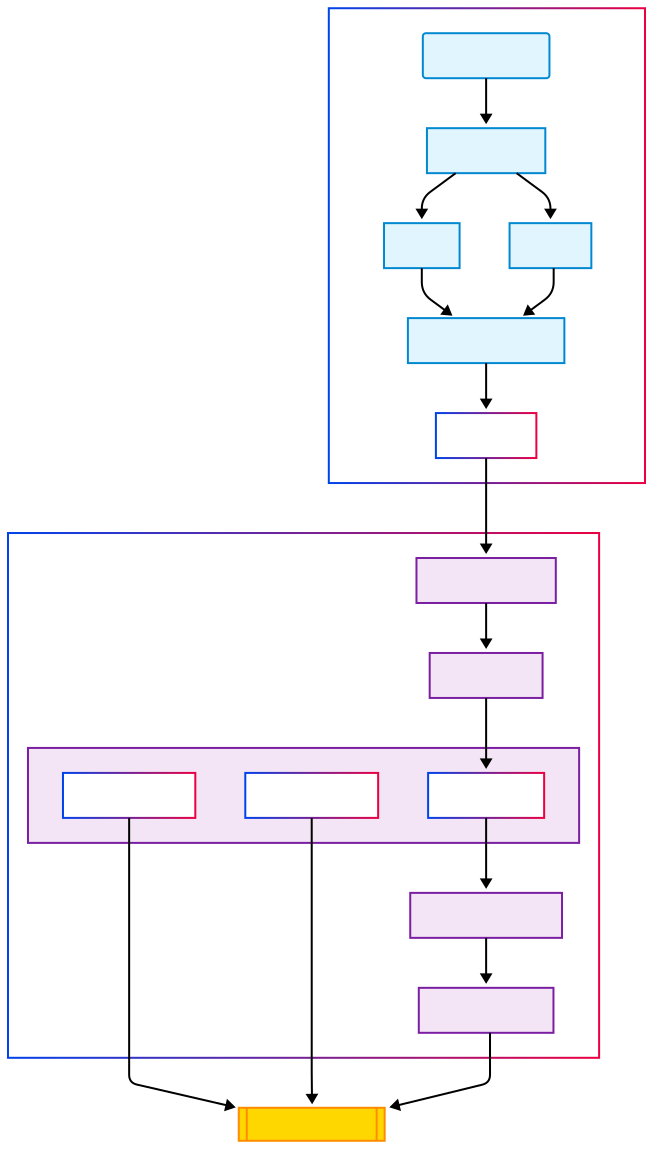
\includegraphics[width=0.85\textwidth]{img/user-diagram-flow}
\caption{High level workflow showing user interaction and data processing}
  \label{fig:user-flow}
\end{figure}

Next.js was chosen because it provides server-side rendering, built-in API routes, and excellent developer experience for building interactive applications. The App Router in Next.js 15 makes it easy to organize different parts of the application (dashboard, pitch pages, authentication) while maintaining clean code structure. This architecture supports the route groups used in the implementation, including `(dashboard)`, `(pitch)`, and `(auth)` directories that separate functional areas without affecting URL routing.

For the backend, Convex was selected after comparing it with traditional databases like PostgreSQL and other backend-as-a-service options. Convex provides real-time data synchronization, built-in schema validation, and server functions that run in the cloud. This eliminates the complexity of managing database connections, implementing real-time updates, or handling server deployment, allowing focus on the evaluation logic.

The authentication layer uses Clerk, which provides complete user management including organizations for multi-tenant data separation. This is important for research applications where different groups need to maintain separate data while using the same system. Clerk handles user registration, login, password management, and organization membership without requiring custom authentication logic.

For GenAI processing, OpenAI's GPT-4 API is used for all evaluation tasks and Whisper for audio transcription. This single-provider approach was chosen after testing multiple alternatives, as it provides the most consistent results while keeping the architecture simple. The system uses GPT-4 for structured evaluation, question generation, and answer processing, while Whisper handles audio file transcription with support for multiple audio formats.

\subsection{Evaluation Framework}\label{subsec:evaluation-framework}

The evaluation framework, developed by analyzing venture capital research and startup success factors, serves as the core mechanism for how Pista assesses startup pitches by identifying the most important evaluation criteria. The framework evaluates pitches systematically across multiple dimensions using standardized criteria and weighted scoring to ensure consistent assessments.

The framework evaluates pitches across four main dimensions, each with specific weights based on their importance for startup success:

\begin{itemize}
  \item \textbf{Problem\mbox{-}Solution Fit}: 0.3
  \item \textbf{Business Model \& Market}: 0.3
  \item \textbf{Team \& Execution}: 0.25
  \item \textbf{Pitch Quality}: 0.15
\end{itemize}

The highest weights were assigned to Problem-Solution Fit and Business Model \& Market because research consistently shows these factors are the strongest predictors of startup success. Team \& Execution receives the next highest weight since execution capability is crucial for converting good ideas into successful businesses. Pitch Quality has the lowest weight because while presentation skills matter for raising capital, they are less predictive of actual business outcomes.

Each dimension evaluates five specific aspects, creating a comprehensive 20-aspect evaluation framework. For example, Problem-Solution Fit examines problem definition clarity, solution innovation, market understanding, competitive advantage, and value proposition. This systematic breakdown ensures thorough coverage of all critical elements.

Figure~\ref{fig:eval-flow} illustrates how each pitch moves through the evaluation pipeline. The system analyzes the content against each dimension's criteria using GPT-4, then combines the results using the predetermined weights to calculate final scores.

\begin{figure}[H]
  \centering
  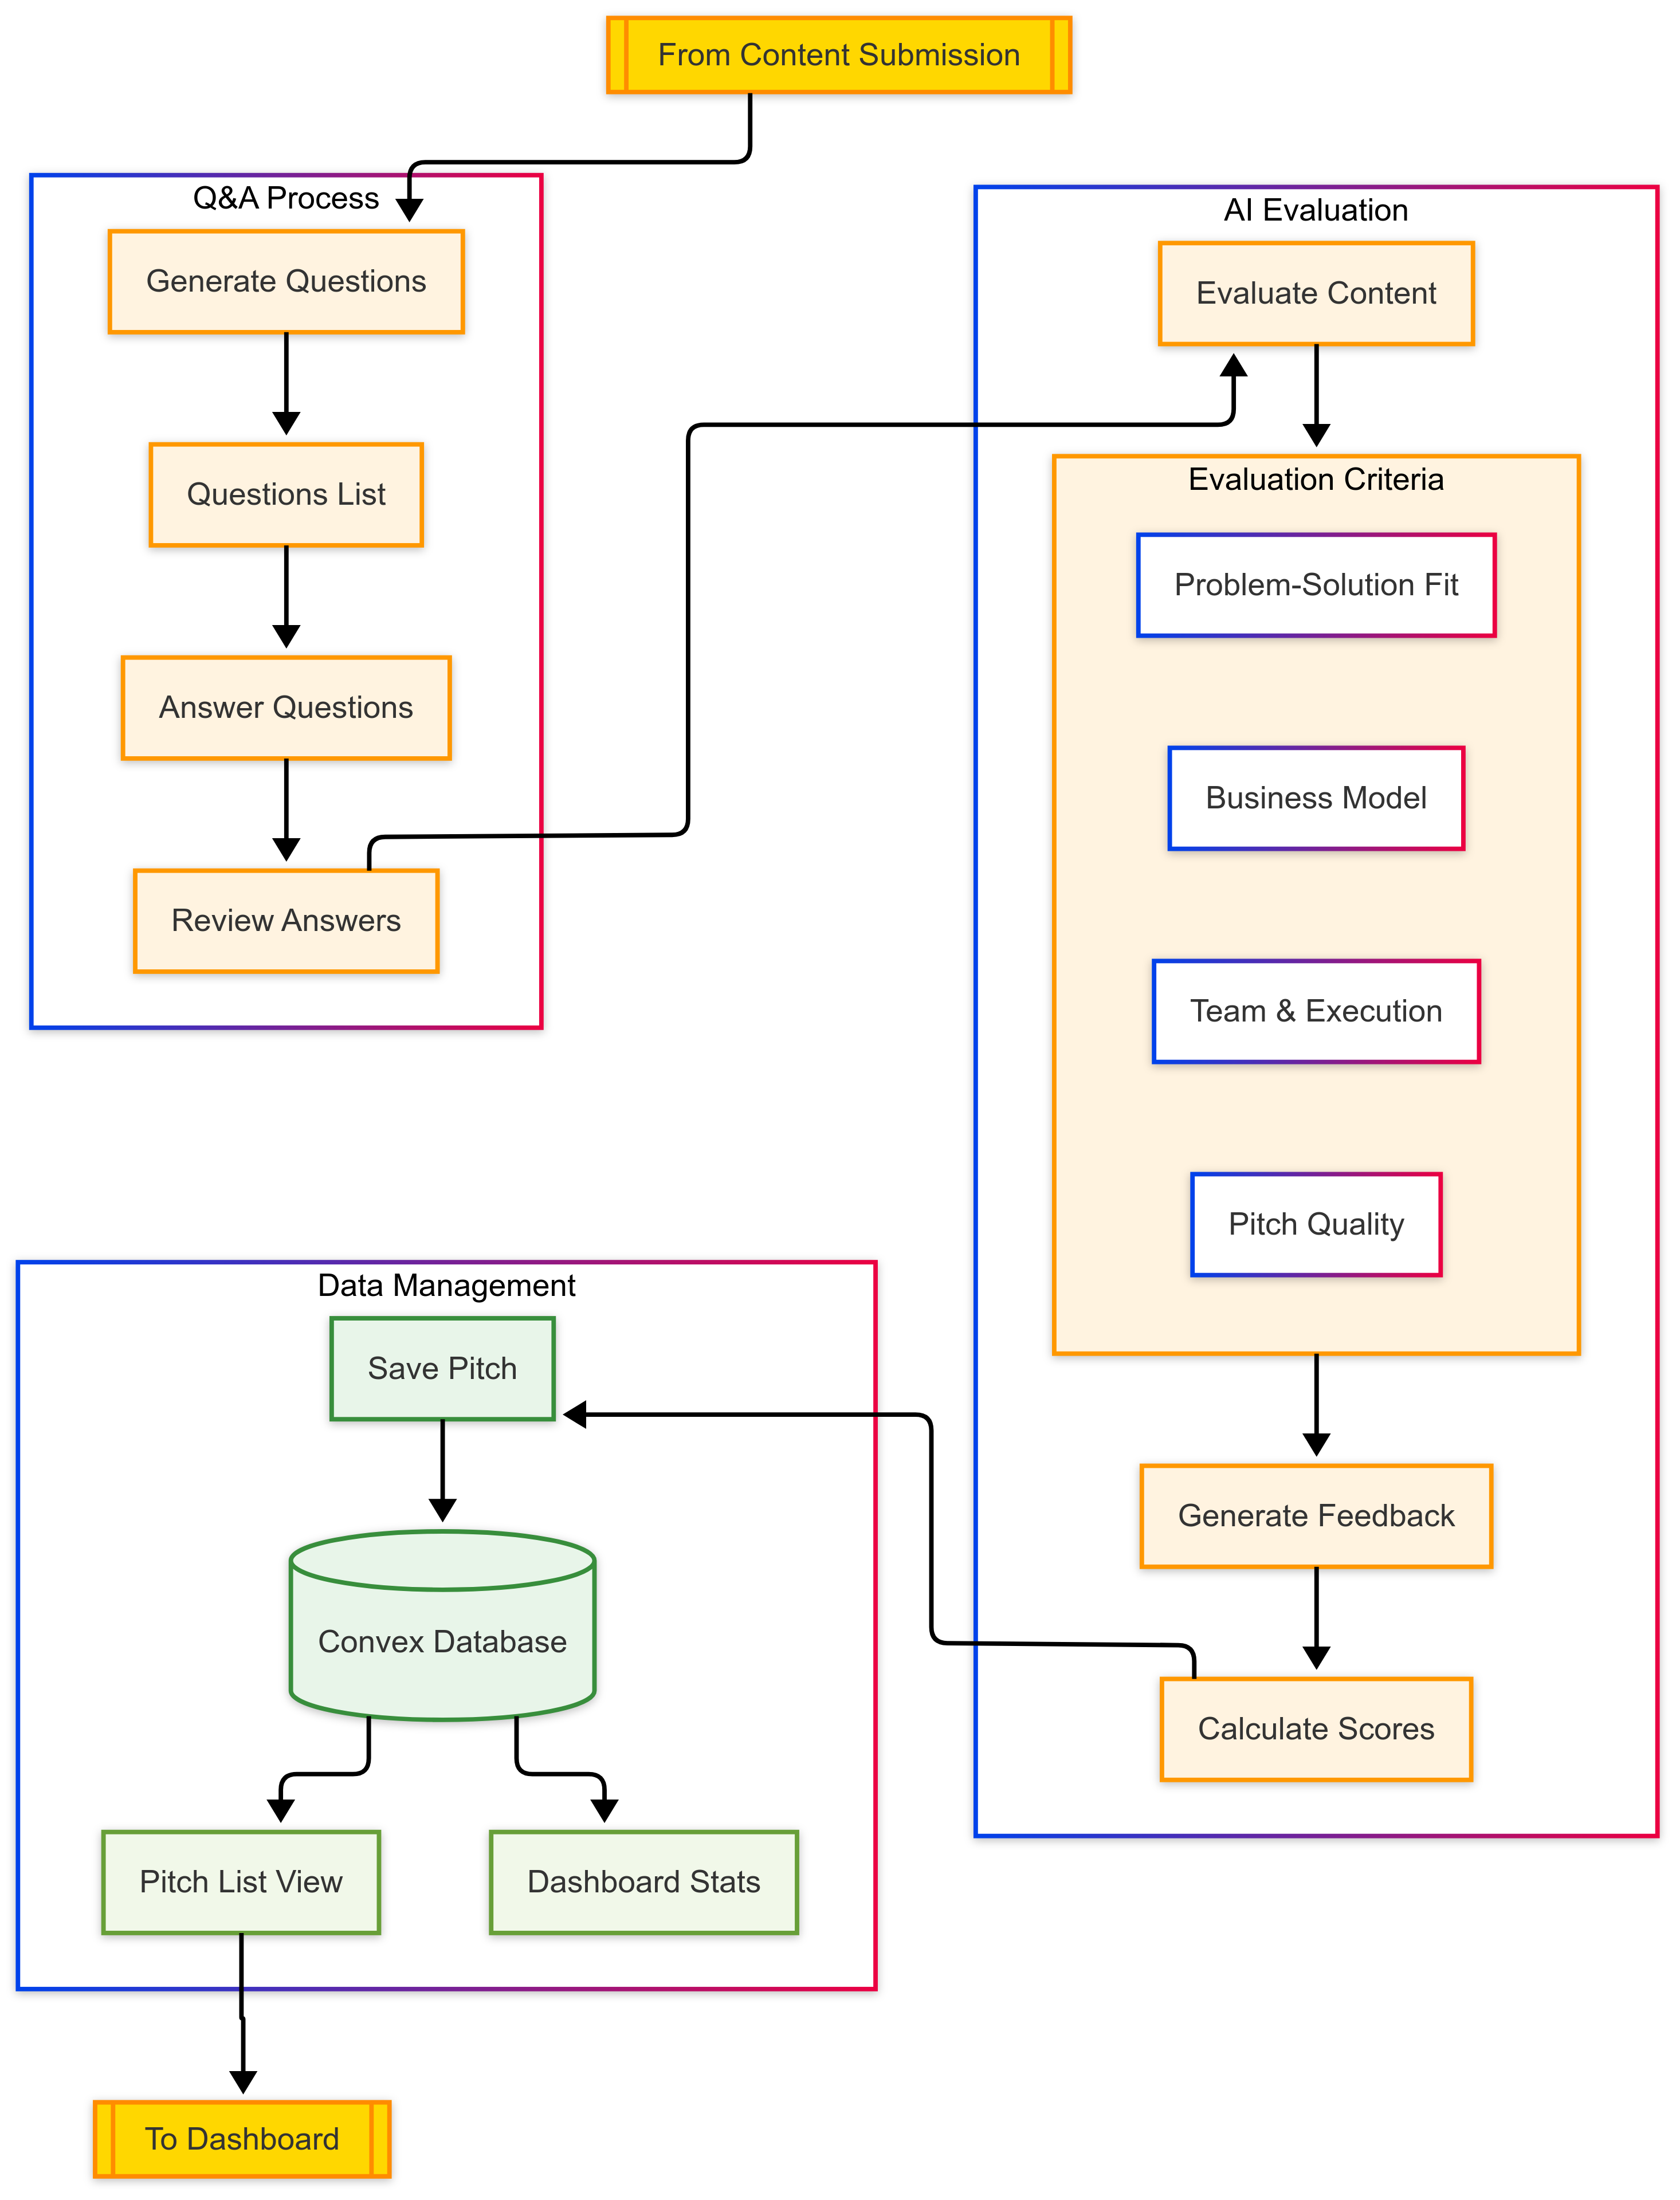
\includegraphics[width=0.9\textwidth]{img/eval-flow}
\caption{Evaluation and processing flow across four criteria}
  \label{fig:eval-flow}
\end{figure}

The scoring system uses a 1-10 scale with specific rubric anchors to ensure consistent evaluation; evidence-based scoring rules were implemented to prevent pitches from receiving high scores without supporting data. The rubric anchors define clear requirements for each score level:

\begin{enumerate}
    \item \textbf{Scores 1--2}: No concrete evidence, claims only
    \item \textbf{Scores 3--4}: Weak or indirect evidence, plan not validated
    \item \textbf{Scores 5--6}: Mixed evidence, partial validation or unclear metrics
    \item \textbf{Scores 7--8}: Strong evidence, credible metrics, risks addressed
    \item \textbf{Scores 9--10}: Exceptional evidence, repeated traction, benchmarks exceeded
\end{enumerate}

This evidence-gating approach addresses the central tendency problem where evaluations cluster around mid-scale scores without meaningful discrimination between pitch quality levels. The rubric was developed through iterative testing to ensure scores reflect actual business validation rather than presentation quality alone. These scoring rules prevent unsupported claims from receiving high ratings while rewarding pitches with concrete evidence of market traction and business validation.

Listing~\ref{lst:eval-criteria} shows how the evaluation criteria and weights were implemented as TypeScript constants to ensure consistency across all assessments.

\begin{lstlisting}[
  language=TypeScript,
  caption={Evaluation criteria and weights implementation},
  label=lst:eval-criteria,
  basicstyle=\footnotesize\ttfamily,
  breaklines=true
]
const EVALUATION_CRITERIA = {
  problemSolution: {
    name: "Problem-Solution Fit",
    aspects: [
      "Problem Definition Clarity",
      "Solution Innovation",
      "Market Understanding",
      "Competitive Advantage",
      "Value Proposition",
    ],
  },
  businessModel: {
    name: "Business Model & Market",
    aspects: [
      "Revenue Model",
      "Market Size & Growth",
      "Go-to-Market Strategy",
      "Customer Acquisition",
      "Scalability Potential",
    ],
  },
  team: {
    name: "Team & Execution",
    aspects: [
      "Team Capability",
      "Domain Expertise",
      "Track Record",
      "Resource Management",
      "Implementation Plan",
    ],
  },
  presentation: {
    name: "Pitch Quality",
    aspects: [
      "Clarity & Structure",
      "Data & Evidence",
      "Story & Engagement",
      "Q&A Performance",
      "Overall Persuasiveness",
    ],
  },
} as const;

const WEIGHTS: Record<string, number> = {
  "Problem-Solution Fit": 0.3,
  "Business Model & Market": 0.3,
  "Team & Execution": 0.25,
  "Pitch Quality": 0.15,
};
\end{lstlisting}

This implementation ensures every evaluation follows exactly the same criteria and weighting scheme. The criteria are defined as constants to prevent runtime modifications and maintain evaluation consistency. The TypeScript type system enforces proper usage of these constants throughout the codebase, preventing inadvertent changes to evaluation criteria during development.

\clearpage
\subsection{GenAI Integration Strategy}\label{subsec:genai-integration-strategy}

GPT-4 was integrated as the core evaluation engine after systematic testing showed it provided the most consistent and high-quality assessments. The integration uses structured prompts that return constrained JSON responses, ensuring reliable data parsing and consistent formatting. All API interactions include strict JSON schema validation to prevent malformed responses from corrupting evaluation data.

The prompt engineering process involved several iterations to optimize evaluation quality. Early testing identified a central tendency problem, where evaluations clustered around 7 out of 10, failing to discriminate between pitches of different quality levels. This was solved by implementing evidence-based scoring rules and rubric anchors.

Listing~\ref{lst:main-eval-prompt} shows the main evaluation prompt template that was developed for structured assessment:

\begin{lstlisting}[
  language=TypeScript,
  caption={Main evaluation prompt template for structured assessment},
  label=lst:main-eval-prompt,
  basicstyle=\footnotesize\ttfamily,
  breaklines=true
]
function buildStructuredPrompt(
  criteriaName: string,
  aspects: string[],
  fullContent: string
): string {
  return `
As an expert evaluator, score ONLY the criterion: ${criteriaName}.

Work from the content below without inventing facts. If evidence is
missing for an aspect, score that aspect <= 4 and note what is missing.

Aspects to score (each 1-10 with a one sentence rationale):
${aspects.map((aspect) => `- ${aspect}`).join("\n")}

Content to evaluate (pitch + Q&A):
${fullContent}

${RUBRIC_ANCHORS}

JSON response schema (valid JSON only):
{
  "score": 1-10, // criterion score = rounded average of aspectScores[].score
  "strengths": [{ "point": "...", "impact": "High"|"Medium"|"Low"}],
  "improvements": [{ "area": "...", "priority": "Critical"|"Important"|"Nice to Have", "actionable": "..."}],
  "aspectScores": [
    { "aspect": "${aspects[0]}", "score": 1-10, "rationale": "..." },
    { "aspect": "${aspects[1]}", "score": 1-10, "rationale": "..." },
    { "aspect": "${aspects[2]}", "score": 1-10, "rationale": "..." },
    { "aspect": "${aspects[3]}", "score": 1-10, "rationale": "..." },
    { "aspect": "${aspects[4]}", "score": 1-10, "rationale": "..." }
  ],
  "summary": "2-3 sentence synthesis",
  "recommendations": ["actionable step 1", "actionable step 2"]
}

${SCORING_RULES}
`;
}
\end{lstlisting}

This prompt template enforces evidence-based evaluation by explicitly instructing the model to avoid inventing facts and to cap scores at 4 when supporting evidence is missing. The structured JSON response ensures consistent data format across all evaluations.

A separate question generation system was also implemented to identify information gaps in pitch content. This system analyzes the pitch and generates up to 3 targeted questions that would materially improve evaluation quality if answered. The questions focus on specific evidence gaps that prevent confident evaluation rather than general business development advice.

\clearpage
Listing~\ref{lst:question-prompt} shows the question generation prompt:

\begin{lstlisting}[
  language=TypeScript,
  caption={Question generation prompt for evidence gathering},
  label=lst:question-prompt,
  basicstyle=\footnotesize\ttfamily,
  breaklines=true
]
const prompt = [
  `Analyze the following pitch and identify the most important gaps that prevent a confident evaluation. Select up to 3 questions that, if answered, would materially improve the assessment.`,
  `Pitch:\n"${truncate(text, MAX_PROMPT_CHARS)}"`,
  `\nReturn valid JSON only with this schema:\n{\n  "items": [\n    {\n "dimension": "Problem-Solution Fit" | "Business Model & Market" | "Team & Execution" | "Pitch Quality",\n      "question": "one specific question, no multi-part prompts",\n      "why_needed": "why this matters for evaluation",\n      "suggested_format": "how to answer: numbers, metrics, bullets, examples",\n      "priority": "Critical" | "Important"\n    }\n  ]\n}\n\nConstraints:\n- Ask 1-3 questions total.\n- Make each question specific and evidence-seeking.\n- Do not request sensitive data.\n- Avoid duplicates and multi-part questions.`,
].join("\n\n");
\end{lstlisting}


This question generation approach systematically identifies evidence gaps before conducting the final assessment, improving evaluation accuracy while ensuring questions remain answerable within a typical pitch context. The system constrains questions to avoid requesting sensitive data or internal documentation that would not be available in standard pitch scenarios. Each generated question includes priority levels and suggested answer formats to guide users toward providing the most valuable additional information for evaluation improvement.

For reliability, exponential backoff retries were implemented for API interactions and strict JSON validation before data persistence. The system uses a low temperature setting (0.2) for all evaluation requests to reduce randomness while maintaining appropriate response variation. Error handling includes comprehensive logging for debugging while ensuring user-facing error messages remain clear and actionable without exposing system internals.

\subsection{Data Models and Storage Architecture}\label{subsec:data-models-and-storage-architecture}

The data architecture was designed to support both real-time user interactions and research data collection. Convex combines database functionality with built-in schema validation and real-time synchronization. Convex provides automatic schema enforcement and type safety that prevents data corruption while eliminating the need for separate database migration management.

The main data model centers around the \texttt{`pitches`} table, which stores essential pitch information including title, content, submission type, processing status, structured evaluation results, question-answer pairs, and organizational metadata. Each document is automatically scoped by user and organization identifiers, providing secure data isolation for multi-tenant use.

The database schema implements several indexes to optimize query performance: \texttt{`by\_org`}, \texttt{`by\_user`}, \texttt{`by\_user\_org`}, and \texttt{`search\_title`}. The data model stores both structured evaluation results and complete audit trails for research reproducibility. Question-and-answer pairs are stored with each pitch and reused when building evaluation input, allowing systematic gathering of additional context that improves assessment quality. The system stores structured evaluation data with detailed scoring breakdowns and improvement recommendations for comprehensive analysis.

\subsection{API Endpoints and Server Functions}\label{subsec:api-and-server}

The API architecture uses Next.js API routes for GenAI processing and Convex functions for data management. This separation allows each component to be optimized for its specific computational requirements. Next.js API routes handle external integrations with OpenAI, while Convex functions manage all database operations with built-in real-time synchronization.

The GenAI processing endpoints include:
\begin{itemize}
  \item \texttt{/api/evaluate}: Processes pitch text using GPT-4 for comprehensive evaluation
  \item \texttt{/api/generate-questions}: Produces targeted follow-up questions using evidence-gap analysis
  \item \texttt{/api/transcribe}: Handles audio file transcription using OpenAI's Whisper model
  \item \texttt{/api/evaluate-answers}: Supports evaluation updates based on question responses
\end{itemize}

These endpoints run on Vercel's Edge runtime for improved performance and global distribution. All API responses are validated against strict schemas before data persistence to ensure research data integrity.

The Convex functions handle all data lifecycle operations including create, update, remove, favorite, unfavorite, and export operations. Query functions support diverse access patterns needed for both user interface functionality and research data analysis, including filtered searches, statistics, and CSV export for external analysis.

\section{Authentication and Authorization Implementation}

The authentication system uses Clerk to provide complete user management with multi-tenant organization support. This design ensures secure data isolation between different research groups while maintaining a simple security model. The implementation includes Next.js middleware that protects dashboard routes and redirects unauthenticated users to the sign-in page. Security headers are applied to all responses through the middleware layer, providing additional protection against common web vulnerabilities. The Clerk integration handles user registration, login, password management, and organization membership without requiring custom authentication logic, reducing security risks while maintaining a professional user experience.


\section{User Interface Implementation}

The user interface was built using Next.js 15 with React 18 and Tailwind CSS to provide a responsive, modern experience optimized for research applications. The application was organized using route groups to separate functional areas: dashboard for pitch management, individual pitch pages for detailed evaluation views, and authentication areas.

Figure~\ref{fig:dashboard} shows the main dashboard interface, which provides an overview of all pitch submissions with evaluation scores, search and filtering capabilities, and direct access to detailed results.

\begin{figure}[H]
  \centering
  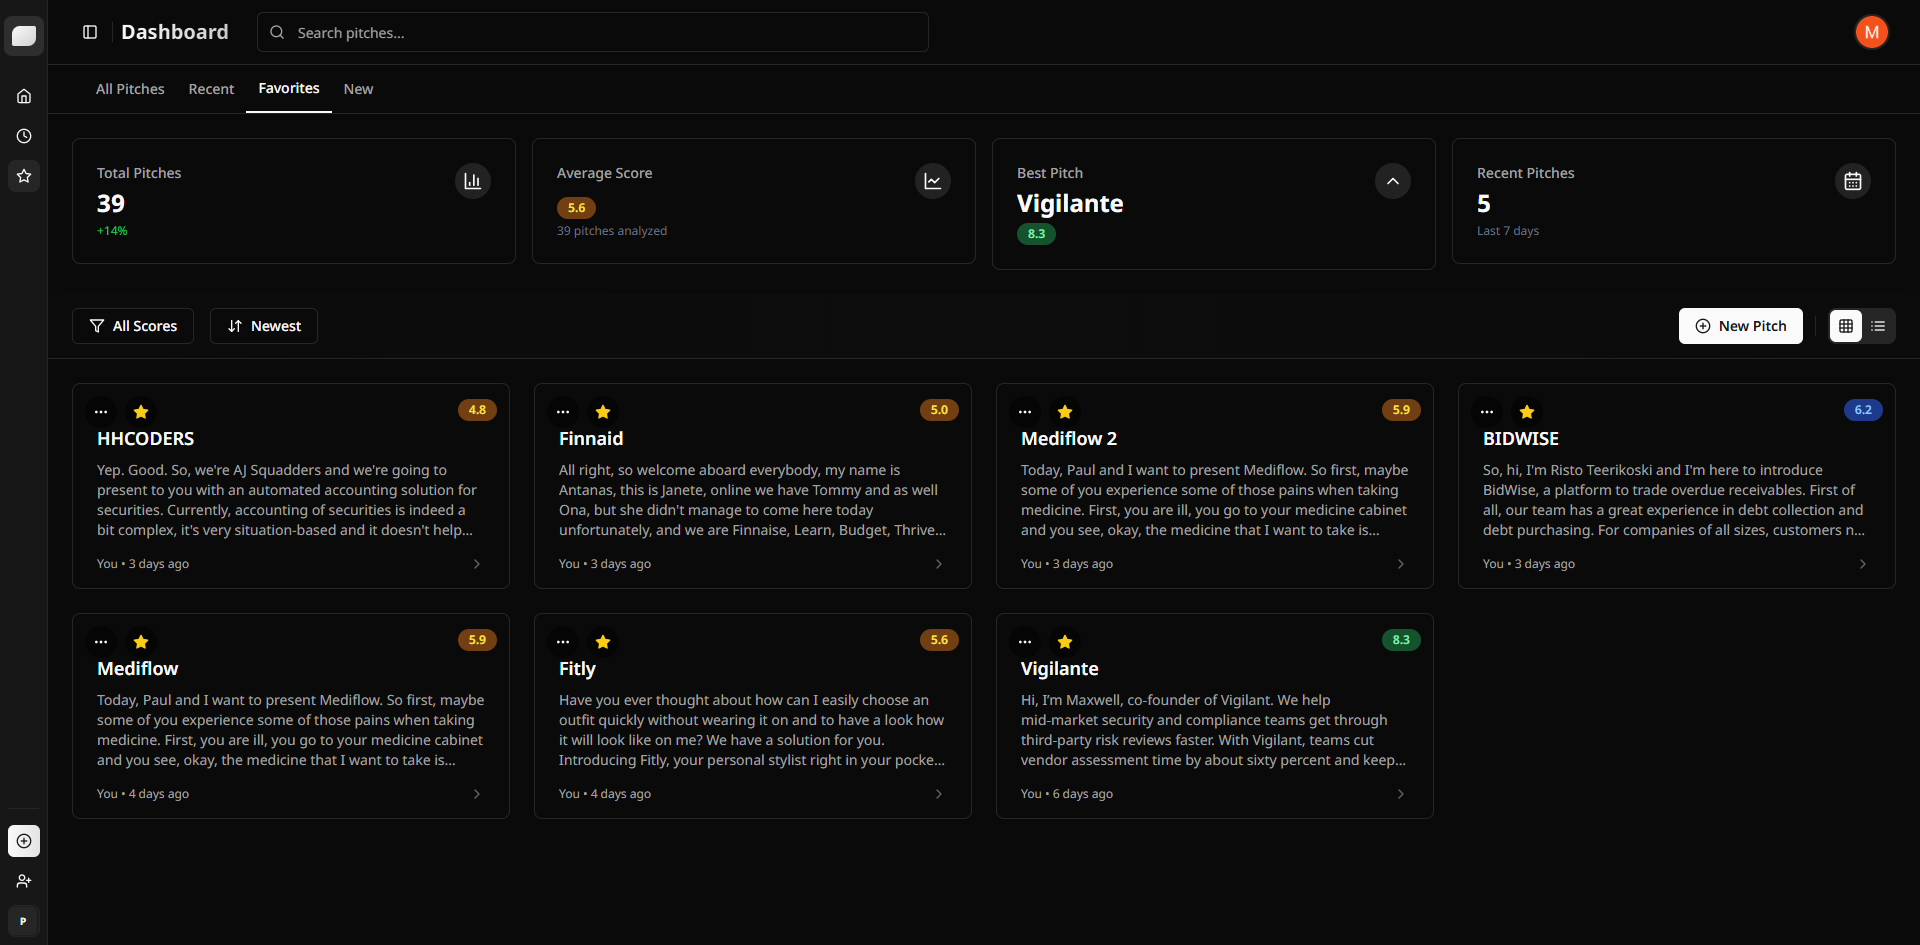
\includegraphics[width=0.9\textwidth]{img/dashboard}
\caption{Main dashboard interface showing pitch management and evaluation scores}
  \label{fig:dashboard}
\end{figure}

The component architecture separates shared UI primitives from feature-specific components to promote reusability and consistent design patterns. The dashboard implements comprehensive list management with user favorites, text-based search, and filtering by evaluation scores or submission dates. Components are organized into logical directories with 'src/components/ui/' containing base components and 'src/components/shared/' housing feature-specific components grouped by domain, including navigation, forms, modals, and authentication. The multi-step pitch upload process uses a dedicated component hierarchy in `src/components/shared/forms/add-pitches/steps/` that manages state progression, validation, and user guidance throughout the evaluation workflow. This architectural separation ensures consistent design language while enabling independent development and testing of complex features like the question generation and evaluation display components.

Figure~\ref{fig:user-flow-pitch} illustrates the pitch creation workflow that was designed to guide users through the evaluation process efficiently. The flow handles both text input and audio file uploads, manages question generation and response collection, and performs evaluation processing with complete metadata storage.

\begin{figure}[H]
  \centering
  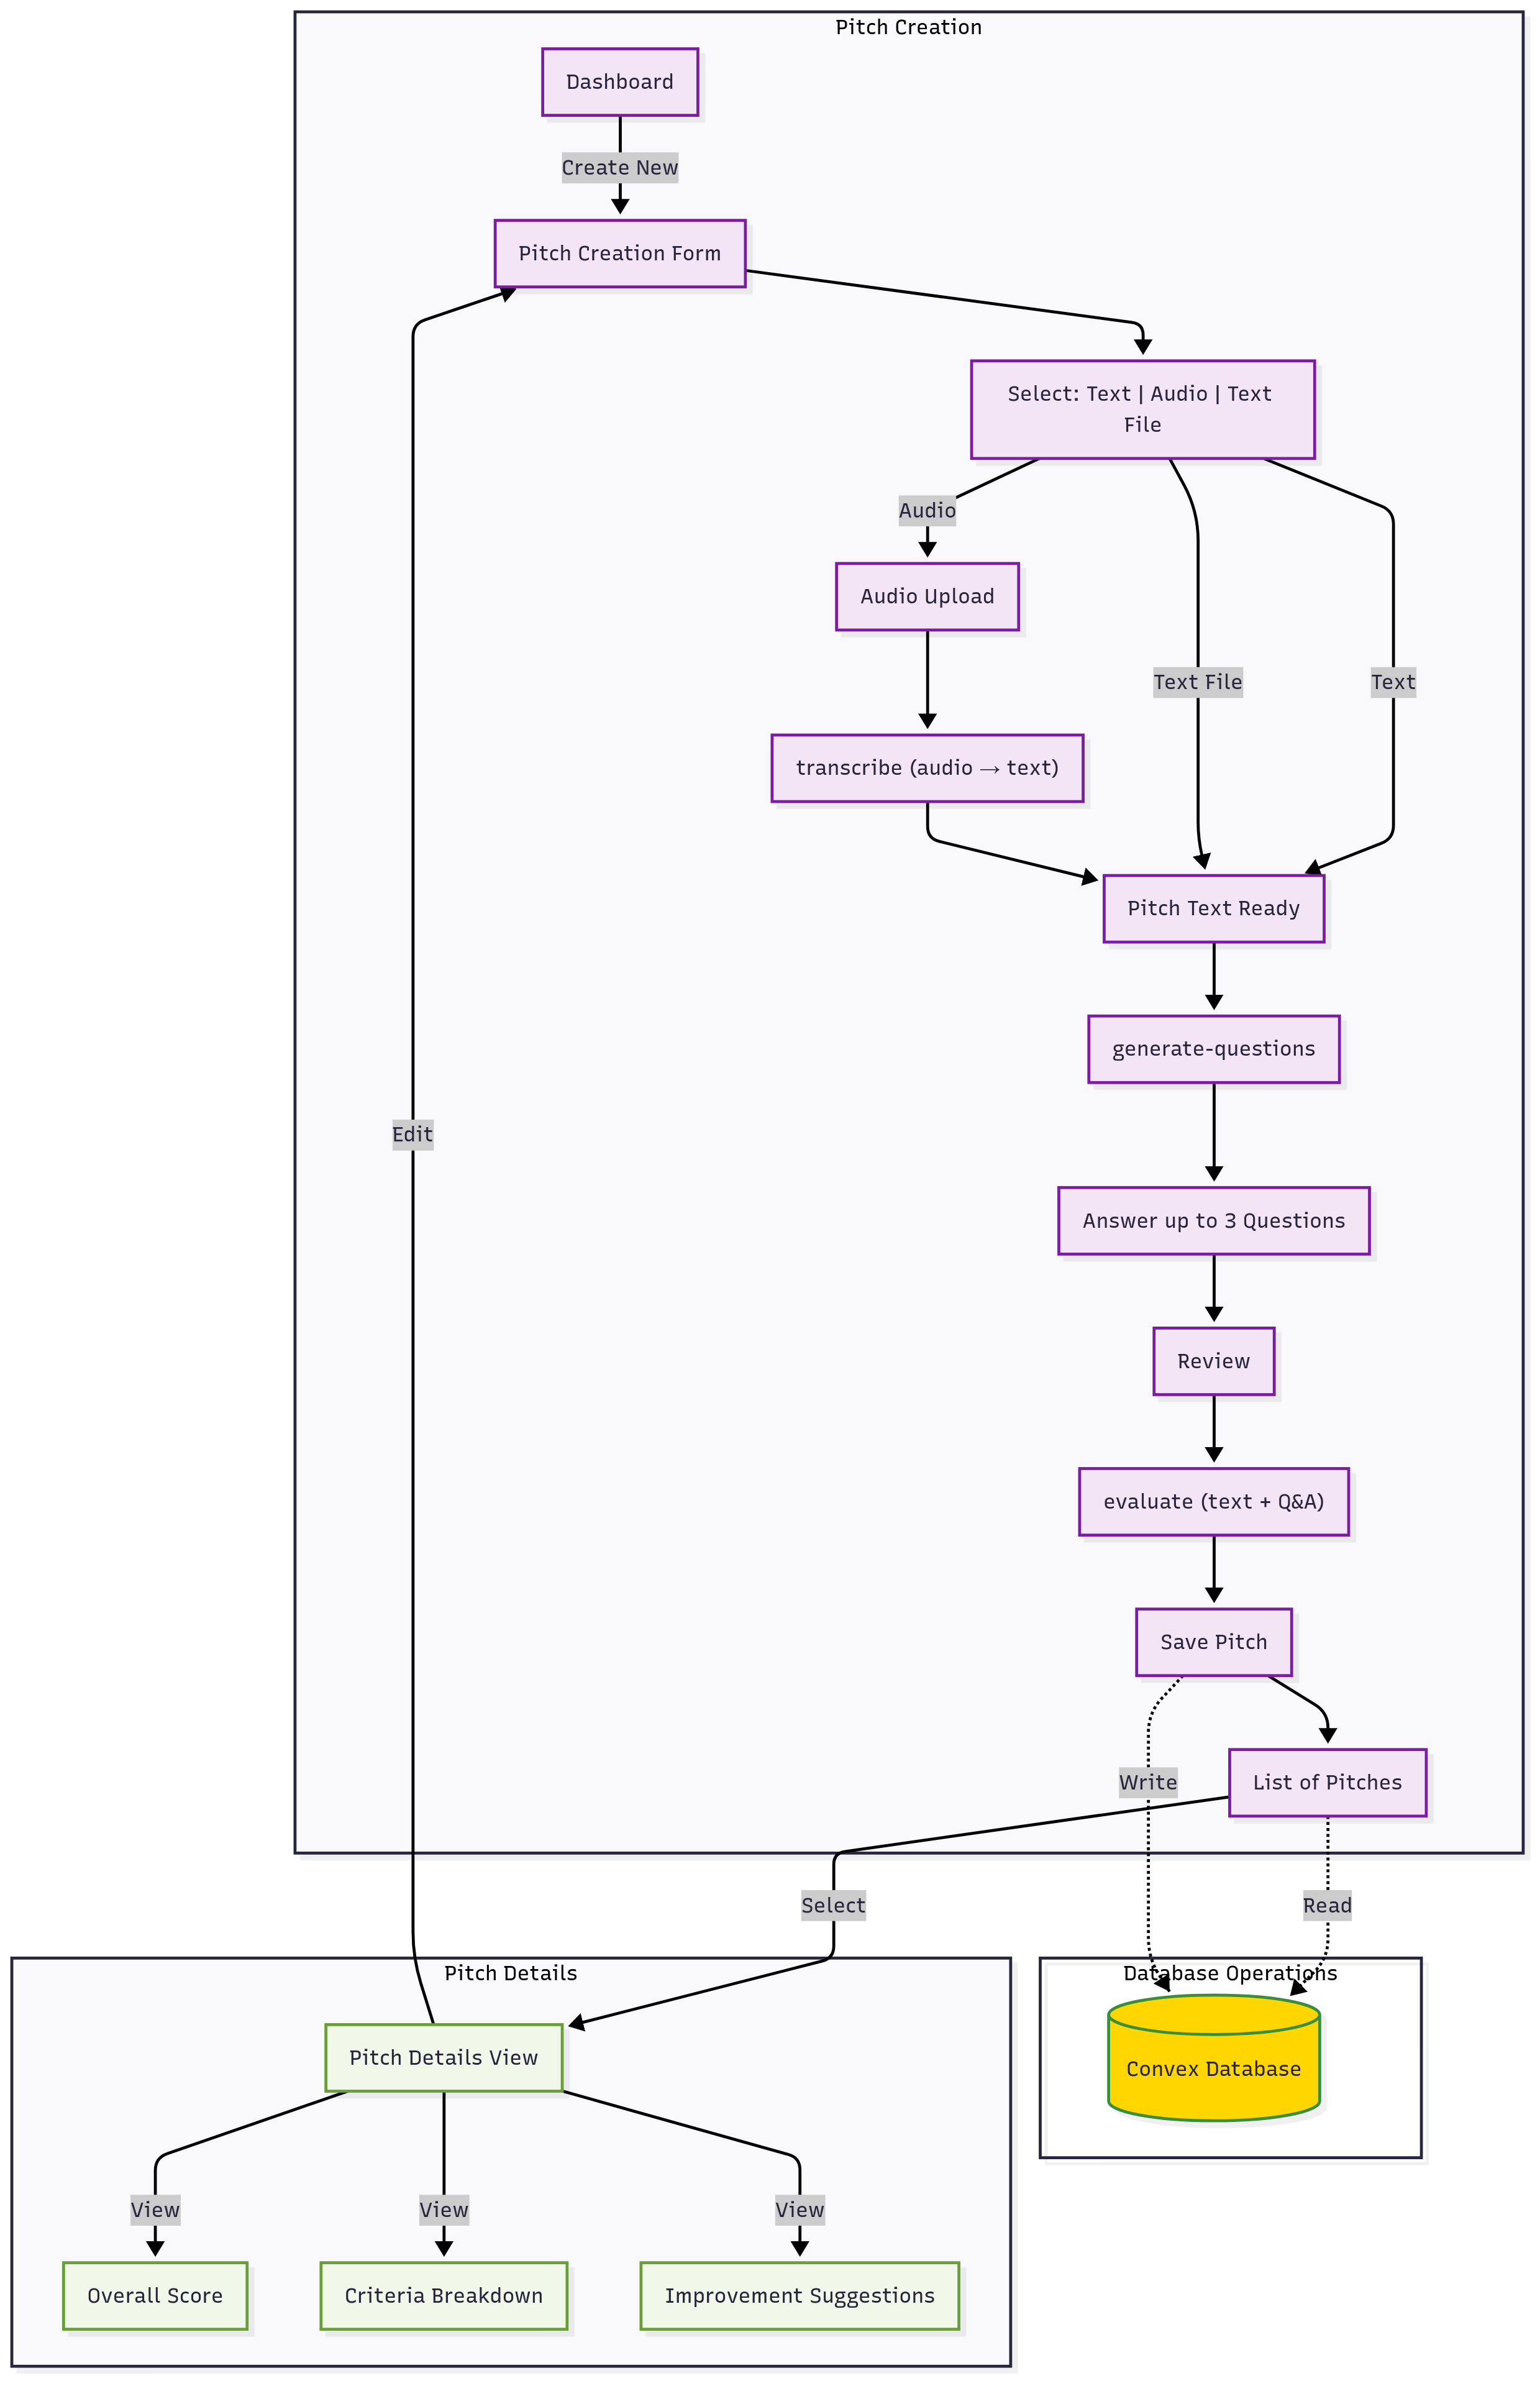
\includegraphics[width=0.9\textwidth]{img/user-flow-pitch}
\caption{Pitch creation flow with Q\&A generation and Convex storage}
  \label{fig:user-flow-pitch}
\end{figure}

The question-and-answer step is optional but enabled by default based on testing that showed significant evaluation quality improvements. Users can skip this step for faster processing, though this may result in less comprehensive evaluations when key information is missing from the original pitch. The questions component implements a multi-step interface that presents one question at a time with visual progress indicators, helping users maintain focus while providing targeted responses that address specific evaluation criteria gaps. The system dynamically generates up to three questions using GPT-4's analysis of the pitch content, with each question targeting critical missing information needed for accurate assessment. The component includes explanatory text stating ``\textit{These questions help improve your evaluation accuracy}'' to guide user understanding of the purpose and value of providing additional context during the evaluation process.

The individual pitch view renders both numeric scores and qualitative feedback alongside generated follow-up questions, providing users with complete evaluation information in a clear, structured format optimized for review and improvement planning. The pitch page implementation uses lazy loading to optimize performance by loading components such as `ScoreOverview`, `EvaluationSummary`, `DetailedAnalysis`, and `QuestionsSection` only when needed, while maintaining responsive skeleton placeholders during content loading. The system supports both legacy and structured evaluation formats through conditional rendering that automatically detects the evaluation data type and displays the appropriate analysis components. This modular architecture enables rich data visualization with transcript sections, comprehensive score breakdowns, and targeted improvement recommendations while maintaining fast initial page loads and smooth user interactions throughout the evaluation review process.

\section{Performance, Deployment, and Reliability}

System performance was optimized to handle the computational demands of GenAI processing while maintaining responsive user interactions. The implementation uses virtualized lists to maintain interface responsiveness with large datasets, code splitting to reduce initial page load times, and reactive queries that eliminate manual polling by automatically updating the interface when results become available.

The deployment architecture uses Vercel for hosting with environment variables for configuration, including database URLs, authentication keys, and API credentials. Critical API routes run on Vercel's Edge runtime for global distribution and reduced latency. The deployment pipeline ensures identical code paths across development and production environments to maintain evaluation result consistency.

For reliability, comprehensive error handling was implemented throughout the system. API routes return clear, actionable error messages that help users resolve problems without exposing sensitive system details. The system includes exponential backoff retries for external API interactions and strict JSON validation before data persistence to prevent corrupted evaluations from entering the research database.

\section{Implementation Results and User Experience}\label{sec:results}

The implemented system achieves the design goals of providing consistent, evidence-based startup pitch evaluations. Text-based pitch evaluations typically complete within 30 to 60 seconds, providing timely feedback without disrupting research workflows. Audio-based submissions require additional processing time for transcription but remain within acceptable bounds for practical use.

The user interface provides immediate visual feedback throughout the evaluation process with real-time updates that make data changes visible without manual page refreshes. The system maintains responsive performance during concurrent usage, supporting both individual use and classroom scenarios where multiple students submit pitches simultaneously.

The systematic development approach ensured all components integrate properly while maintaining research data integrity. The evidence-based evaluation framework successfully addresses the central tendency problem identified in initial testing, producing meaningful score distributions that discriminate between pitches of different quality levels.

The complete implementation represents a working system that combines GenAI capabilities with research-quality data collection, providing both immediate user value and a foundation for continued evaluation  research.